\documentclass[11pt]{article}
\usepackage[utf8]{inputenc}
\usepackage{fourier}
\usepackage{natbib}
\usepackage[top=2.7cm, bottom=2.7cm, left=2.5cm, right=2.5cm]{geometry}
\usepackage{graphicx}
\usepackage{authblk}
\usepackage{hyperref}
\usepackage{fancyref}

\sloppy

\title{\textbf{Machine Learning and Data Mining with Apache Spark}}
\author{Benjamin Fovet, Maxime Gasque, François Horel, Héloïse Hourquebie, Abderrahman Lahjouji, Anass Seddiki}
\affil{\texttt{\{bfovet, mgasque, fhorel, hhourquebie, alahjouji, aseddiki\} @enseirb-matmeca.fr}}
\date{}

\begin{document}

\maketitle

\textbf{Abstract.} This paper deals with the concepts of \textbf{\textit{machine learning}} and \textbf{\textit{data mining}} social networks, which are increasingly useful for businesses to know the consumers' sentiment towards their brand. This project, intended for use by engineers at Orange France, focuses on the development of a micro-services architecture built around the open source cluster computing framework Apache Spark. Thanks to is distributed model, Spark can process massive amounts of data stored in databases as well as real time data streamed from social networks such as Twitter, Facebook and Orange forum websites. These data are then stored in a cluster database and exposed by an Application Programming Interface (API) server for users to see them in real time.


\section{Context}
% What is Big Data ? (short intro)
Big data is a term used to designate data that is not only too voluminous to fit in a standard database, but is also too diverse and appears at such speed that it cannot be processed using mainstream systems. [Big data now, 2012 edition]

% Orange wants to use Apache Spark
Currently, Orange France is a company already working on big data applications and is interested in using emerging big data technologies. More precisely, among those technologies available today, Apache Spark is the most promising one thanks to its processing performances that makes it well suited to machine learning algorithms.

% What is Apache Spark ? What are the possibilities ? How does it work ?
\subsection{Apache Spark}
\label{apache spark}
Apache Spark is a distributed and highly scalable in-memory system, providing the ability to develop applications using languages like Java, Scala (the language used to write Spark itself), Python and R. It was originally developed at the University of California, Berkeley and donated to the Apache Software Foundation in 2013.
Spark actually consists of four main interoperable components. The figure \ref{spark-stack} below shows the modules built on top of the Spark Core.

\begin{figure}[h!]
    \centering
    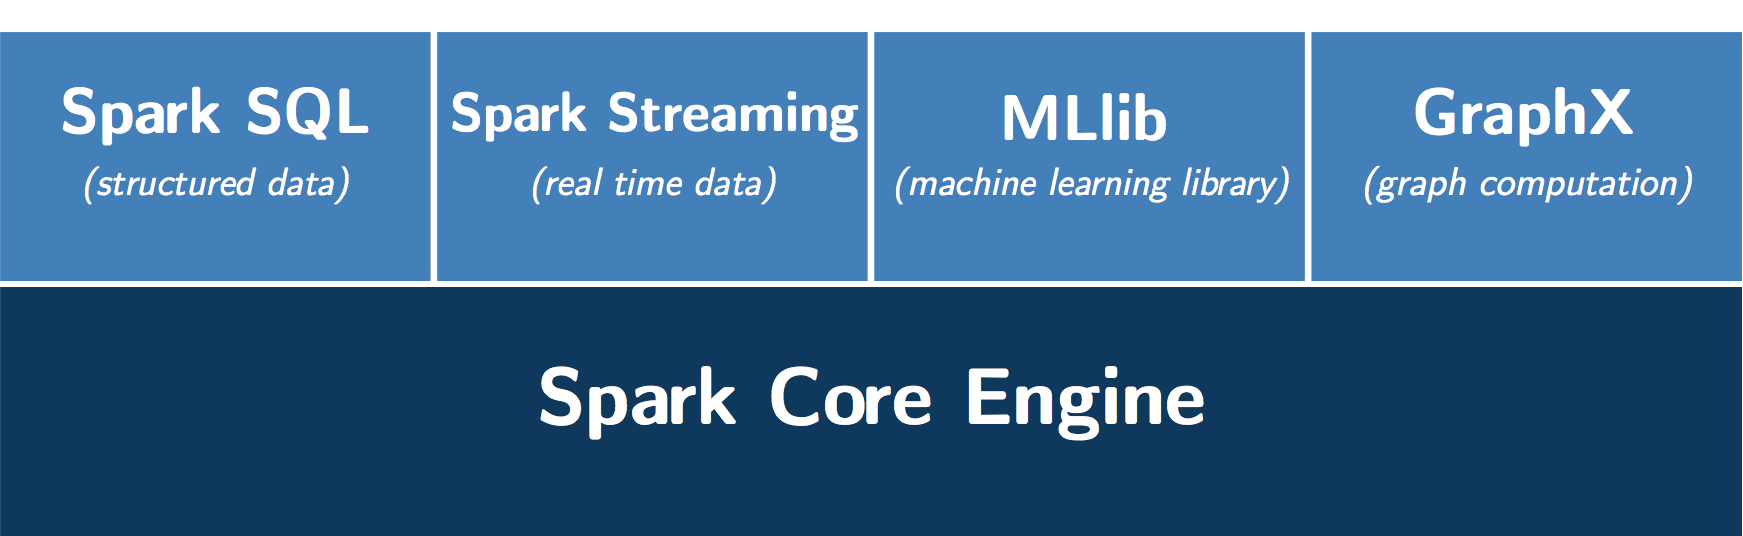
\includegraphics[scale=0.25]{img/spark-stack.eps}
    \caption{The Spark stack}
    \label{spark-stack}
\end{figure}

Spark Core is the foundation of the Spark project and contains functionalities such as task scheduling, memory management, fault recovery and more. On top of that lies four submodules.
Spark SQL is Spark's package for working with structured data which allows SQL queries on many sources of data.
Spark Streaming leverages Spark Core capabilities to enable processing of live streams of data. It is used extensively in this project for fetching data from social networks.
MLlib is a library containing machine learning algorithms that can be applied to compute statistical models from data.
Finally, GraphX is another library for manipulating graphs and performing graph computations.

% Our goal is to demonstrate Spark capabilities, effectiveness and usability through use cases
\subsection{Using Spark in real world scenarios}
The goal of this project is to demonstrate Spark capabilities, effectiveness and usability. At first, requirements were not clearly defined as this project is mainly aimed at exploring what can be done with Spark, but they had to match certain expectations from Orange. These requirements, introduced in the next section, take the shape of use cases as well as Spark integration with other tools.

\section{Developed use cases}
% Video use case
\subsection{Estimating the crowd in Orange stores}

% Social networks use case
\subsection{Data mining social networks}

\subsubsection{Identifying useful sources}

Social networks are a highly valuable source of information about consumers relationship towards a brand. For instance, Orange uses Facebook through two pages: \href{https://www.facebook.com/Orange.France/?ref=ts}{\textbf{Orange}} and \href{https://www.facebook.com/sosh/?fref=ts}{\textbf{Sosh}}, manages several Twitter accounts: \href{https://twitter.com/orange}{\textbf{@orange}} and \href{https://twitter.com/Orange_France}{\textbf{@Orange\_France}} for general communication about Orange, \href{https://twitter.com/Sosh_fr}{\textbf{@Sosh\_fr}} and \href{https://twitter.com/Orange_conseil}{\textbf{@Orange\_conseil}} as after-sales service accounts. Moreover, consumers can access forums at \href{https://communaute.orange.fr}{\url{communaute.orange.fr}}.

All these sources are used for fetching live data and feeding Spark with them.

\subsubsection{Spark applications}

As said in section~\ref{apache spark}, Spark applications can be written in several languages: Java, Python or Scala. Scala was initially chosen since Spark itself is developed in Scala and it is also less verbose than Java code. Furthermore, Java and Scala applications have the advantage of being compiled and packaged into an \textbf{Uber-JAR}. JAR (Java ARchive) is a package file format used to aggregate class files required for an application to run, and an Uber-JAR is a JAR that not only contains the application code but also embeds its dependencies as well. This way, the application only needs to be submitted with the Uber-JAR file to Spark for it to be run.

Applications are also separated by sources, allowing a more flexible development and release to production as well as a reduction of risks. Indeed, Facebook and Twitter have their own independant API services and having issues with one will not impact the other. This structure also leads to a better bug tracking management with having the bug-free application uninterrupted.

\subsubsection{Sentiment analysis}

Sentiment analysis refers to the use of natural language processing and text analysis to identify and extract subjective information in source materials. It aims to classify the polarity of a given text — whether the expressed opinion is positive, negative, or neutral. 
Based on the source, sentiment analysis is applied to tweets on Twitter, posts on Facebook, and thread titles and messages on forums.

% Also talk about testing http://nlp.stanford.edu/sentiment/ in the first place, only for English tweets

\paragraph{Dictionary-based approach}

The first approach consists of deciding whether a text is positive, negative or neutral by looking at words in isolation, giving positive points for positive words and negative points for negative words found in two separate dictionaries and then summing up these points.

The following workflow example is based on a real tweet from an Orange consumer.

% Figure, tweet text : Ma connexion internet est vraiment très instable en ce moment, j'ai souvent aucun accès a internet, c'est normal @Orange_conseil ?

The first step is to tokenize the text, translating a sentence into a list of independant words. This is done using the \texttt{FrenchTokenizer} \url{https://github.com/stanfordnlp/CoreNLP/blob/master/src/edu/stanford/nlp/international/french/process/FrenchTokenizer.java}, part of the Stanford CoreNLP suite of Natural Language Processing tools. Along with tokenizing a text, common words with no interesting meaning such as "le", "dans", "à" also known as "stop words" are filtered out to produce the following list of meaningful words.

% Figure, processed tweet : connexion, internet, vraiment, instable, moment, souvent, aucun, accès, internet, normal

Next, each word in the above list is looked up in the positive and negative words dictionaries. If found, the weight associated with a negative or positive sentiment, depending on which dictionary the word has been found in, is increased by an increment of one.

Finally, the sentiment for the whole tweet is given by computing the difference between the positive weight and the negative weight. A sentiment score equal to 0 is associated with "NEUTRAL", while positive scores are marked as "POSITIVE" and negative scores as "NEGATIVE".

This method is far from perfect since it gives a sentiment based on separate words instead of the context of a sentence. The sentiment analysis annotator from Stanford CoreNLP \url{https://stanfordnlp.github.io/CoreNLP} was tested before implementing this technique and although it yields more accurate results based on a large grammar treebank, it is only available for English text analysis.

\paragraph{Machine learning-based approach}

Thanks to Spark's Machine Learning library \textit{MLlib}, classification algorithms can be applied to analyze tweets. In this approach, the Naive Bayes algorithm, a probabilistic classifier based on Bayes' theorem, is implemented through two steps: train and predict.

Training the data requires having a set of tweets already classified by hand, with 1 meaning positive and 0 meaning negative. This data set is then loaded and split into training data, used to train the classifier model, and testing data, used to assess the performance and the accuracy of the trained model.
With this algorithm, 74\% of the 1343 tweets, is correctly classified.

Predicting is then possible by applying the previous trained model.

\subsubsection{Specific computed indicators}

\paragraph{Twitter}

\paragraph{Facebook}

\paragraph{Orange forums}

% Every component of our architecture
\section{Building a microservices architecture}

% Presentation and schema first

Microservices is an architectural style in which large complex software applications are broken down into a collection of small, independent, loosely coupled processes. This helps upgrading, modifying or changing one service instead of taking down the entire system. As shown in the figure below, this project is composed of several services communicating with each other, which are presented in the next sections.

\subsection{Docker}

To facilitate the deployment of each application, Docker is the ideal technology. It automates the deployment of applications inside containers, isolated from the host and other containers by leveraging functionalities of the Linux kernel. Docker containers wrap up a piece of software in a complete filesystem that contains everything it needs to run: code, runtime, system tools, system libraries – ensuring that it will run consistently across all environments. In terms of virtualization, each Docker container uses the host OS (Linux) features instead of requiring an hypervisor and a guest OS like a virtual machine.

\begin{figure}[h!]
    \centering
    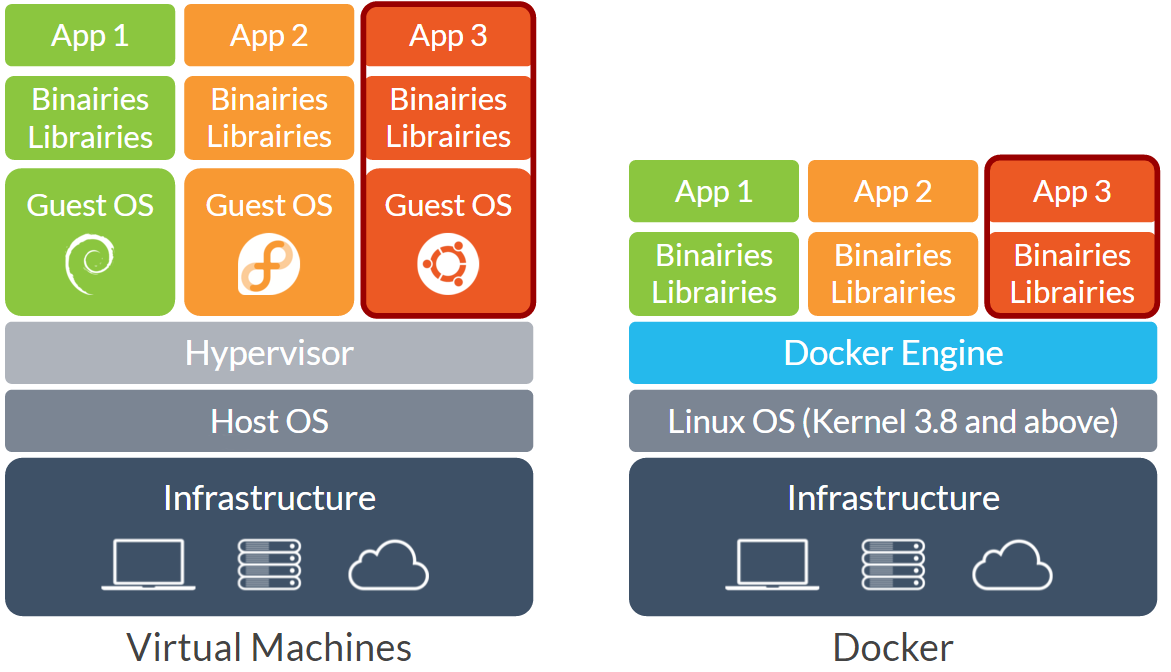
\includegraphics[scale=0.45]{img/docker-vs-vm.png}
    \caption{Comparison between VMs and Docker}
    \label{docker-vs-vm}
\end{figure}

\subsection{Spark cluster}

\subsection{Cassandra database cluster}

\subsection{API}

\subsection{ELK stack}

\section{Organization and Management}

\subsection{Methodology}
\subsection{Tools}
\subsection{Issues}

\section{Conclusion}



\bibliographystyle{plain}
\bibliography{references}

%https://stanfordnlp.github.io/CoreNLP/#citing-stanford-corenlp-in-papers:

Manning, Christopher D., Mihai Surdeanu, John Bauer, Jenny Finkel, Steven J. Bethard, and David McClosky. 2014. The Stanford CoreNLP Natural Language Processing Toolkit In Proceedings of the 52nd Annual Meeting of the Association for Computational Linguistics: System Demonstrations, pp. 55-60. [http://nlp.stanford.edu/pubs/StanfordCoreNlp2014.pdf] [bib]

http://nlp.stanford.edu/publications.shtml:

Richard Socher, Alex Perelygin, Jean Wu, Jason Chuang, Christopher Manning, Andrew Ng, and Christopher Potts. 2013. Recursive Deep Models for Semantic Compositionality Over a Sentiment Treebank. In EMNLP. [pdf, bib, info]

\section{Appendices}
\end{document}